\documentclass[conference]{IEEEtran}
\usepackage[utf8]{inputenc}
\usepackage[T1]{fontenc}
\usepackage{amsmath,amssymb}
\usepackage{graphicx}
\usepackage{booktabs}
\usepackage{algorithm}
\usepackage{algpseudocode}
\usepackage{cite}
\usepackage{xcolor}
\usepackage{url}

\graphicspath{{../figures/}}
% Parts that wait for the full campaign (step 5, issue #14) and its statistics
% (step 6, issues #16 and #21) are marked with \afaire{...}. Remove the macro once filled.
\newcommand{\afaire}[1]{\textcolor{red}{[\textbf{TODO:} #1]}}

\begin{document}

\title{A Massively Parallel Differential Evolution on GPU with CUDA}

\author{
\IEEEauthorblockN{Amina Menacer, Lounis Mesrour, Lisa Adrar}
\IEEEauthorblockA{Master 2 IMDS, Université de Haute-Alsace, Mulhouse, France}
}

\maketitle

\begin{abstract}
Differential Evolution (DE) is a population-based optimizer whose individuals can
build and evaluate their trial vectors independently, which makes it a natural
candidate for graphics processors. Starting from a CUDA implementation of Particle
Swarm Optimization, we design two GPU versions of DE/rand/1/bin and evaluate them
on four shifted benchmark functions (Sphere, Rosenbrock, Griewank, Rastrigin) with a
budget of $10^4 D$ function evaluations. The first version maps one thread to one
individual; no significant difference in solution quality was detected against a
sequential C++ implementation (Mann--Whitney, 10 runs), but it is at most $2.3\times$
faster, because a population of 100 individuals occupies a single streaming
multiprocessor. The second version maps one block to one individual and one thread
to one gene, fuses mutation, crossover, evaluation and replacement into a single
kernel with a shared-memory tree reduction, and keeps the best-individual search on
the GPU. On an NVIDIA Tesla T4 it is $1.7\times$ to $14.6\times$ faster than the first
version, with no significant difference in quality detected, and about $33\times$ faster
than the sequential code on Rastrigin with $D=100$, $N=100$. We also compare five DE variants on the GPU
(three crossover rates, current-to-best/1, and the self-adaptive jDE).
\afaire{final speedups and statistics of the full campaign.}
\end{abstract}

\begin{IEEEkeywords}
CUDA, GPU, Differential Evolution, Massively Parallel Computing, Global Optimization
\end{IEEEkeywords}

% =====================================================================
\section{Introduction}
Population-based metaheuristics spend most of their time evaluating candidate
solutions. In Differential Evolution (DE) \cite{storn1997}, each of the $N$ individuals
produces one trial vector per generation from three other individuals of the
current population; these $N$ constructions and evaluations are independent, and
inside each of them the $D$ coordinates are processed almost independently as well.
This two-level parallelism (individuals, then genes) fits the hierarchy of a GPU
(blocks, then threads).

This work was carried out in the massively parallel computing course of the Master~2
IMDS. The starting point is a CUDA implementation of Particle Swarm Optimization (PSO)
\cite{kennedy1995} provided by the course, which we transform into a DE, following the
approach of Qin et~al.~\cite{qin2012}. Our contributions are:
\begin{itemize}
  \item a diagnosis of the PSO code (race condition on global temporaries, wrong
        Griewank product, missing shift and bounds, best particle computed on the
        CPU at every iteration), which motivated a common, tested interface shared by
        the sequential and GPU programs;
  \item two GPU implementations of DE/rand/1/bin, validated against a sequential
        C++ implementation with statistical tests;
  \item a measured analysis of the block size, occupancy and speedup on a Tesla T4;
  \item a comparison of DE variants (crossover rate, current-to-best/1, jDE \cite{brest2006})
        running on the GPU.
\end{itemize}
Section~\ref{sec:gpu} recalls the CUDA programming model, Section~\ref{sec:de} describes
the sequential and parallel DE, Section~\ref{sec:exp} reports the experiments, and
Section~\ref{sec:conc} concludes.

% =====================================================================
\section{GPU Programming}\label{sec:gpu}
A CUDA GPU is made of streaming multiprocessors (SMs); the Tesla T4 used here has
40 SMs, each running at most 1024 resident threads and offering 48~KB of shared
memory per block. A kernel is launched on a grid of blocks; the threads of a block
run on the same SM, are scheduled by groups of 32 (warps), can synchronize with
\texttt{\_\_syncthreads()} and share a fast on-chip memory. Global memory is large
but slow; it is used efficiently when consecutive threads read consecutive
addresses (coalesced accesses). Constant memory is cached and broadcast to all the
threads of a warp that read the same address. Random numbers are generated on the
device with cuRAND; we use the counter-based Philox generator \cite{salmon2011}, which
gives each thread an independent subsequence of a single seed.

% =====================================================================
\section{Differential Evolution}\label{sec:de}
\subsection{Overview of the sequential DE}
DE/rand/1/bin keeps a population $\{x_1,\dots,x_N\}\subset[\ell,u]^D$. At each
generation, for every individual $i$, three distinct indices $r_1,r_2,r_3\neq i$ are
drawn and a mutant is built:
\begin{equation}
v_i = x_{r_1} + F\,(x_{r_2}-x_{r_3}).
\label{eq:mut}
\end{equation}
Binomial crossover mixes $v_i$ and $x_i$ gene by gene:
\begin{equation}
u_{i,j} = \begin{cases} v_{i,j} & \text{if } \mathrm{rand}_j < CR \text{ or } j=j_{\mathrm{rand}},\\
x_{i,j} & \text{otherwise,}\end{cases}
\label{eq:cross}
\end{equation}
where $j_{\mathrm{rand}}$ guarantees that at least one gene comes from the mutant.
Genes leaving the domain are clipped to $[\ell,u]$. Selection keeps the better of the
two: $x_i \leftarrow u_i$ if $f(u_i)\le f(x_i)$. Unless stated otherwise, we use $F=0.5$ and $CR=0.3$,
and a budget of $10^4 D$ evaluations of $f$, counted exactly (the initial
population costs $N$ evaluations and the last generation may be partial).

The sequential reference (C++, one core) replaces $x_i$ as soon as its trial wins, so
later individuals of the same generation already see the new value. On the GPU the
replacement must take place at the end of the generation (a \emph{generational}
DE), otherwise a thread could read $x_{r_1}$ while another thread overwrites it. The
two programs are therefore two variants of the same algorithm; we compare them
statistically in Section~\ref{sec:exp}.

\subsection{Massively parallel DE}
\paragraph{Common interface} The four functions, their domains, the shift vector $o$
and the CSV format are written once in a header used by the sequential and the GPU
programs (\texttt{\_\_host\_\_ \_\_device\_\_} functions). The shift is generated by a
deterministic generator (splitmix64) seeded with the function and the dimension, so
both programs optimize exactly the same problem. Each function returns the error
$f(x)-f(x^\ast)$, which is $0$ at the optimum.

\paragraph{Version 1 (one thread per individual)} Three kernels per generation:
mutation and crossover into a separate trial array, evaluation of the trials, and
selection. Because trials are written in their own array and selection runs in a
separate kernel, there is no race condition. The shift vector lives in constant
memory and the population never leaves the GPU; only the $N$ final fitness values
are copied back.

\paragraph{Version 2 (one block per individual, one thread per gene)} Two kernels
per generation:
\begin{itemize}
  \item \textbf{kernel P}: one thread per individual draws $r_1,r_2,r_3$ and
        $j_{\mathrm{rand}}$ and stores them as an \texttt{int4};
  \item \textbf{kernel MCER} (Mutation, Crossover, Evaluation, Replacement): block $i$
        builds trial $u_i$ in shared memory, thread $t$ handling genes
        $t, t+T, t+2T,\dots$; each thread computes its part of $f(u_i)$ and the block
        sums them by a tree reduction in $\log_2 T$ steps (Griewank needs a sum and
        a product, reduced together); thread 0 compares with $f(x_i)$ and the block
        writes the winner into a second population buffer.
\end{itemize}
The two population buffers are swapped by exchanging pointers (double buffering),
which removes both the copy and the race condition. The best individual is found by
an argmin reduction kernel (512 threads, ties broken by the smallest index), so the
only transfer inside the timed region is a 16-byte structure. Consecutive threads read
consecutive genes, so global-memory accesses are coalesced, whereas in version~1
threads read with a stride of $D$.

\paragraph{Block size} The number of threads per block $T$ (a power of two) is chosen
automatically: $T=32$ if $D\le 32$ or $N\ge 4\times\#\mathrm{SM}$, and $T=64$
otherwise. The rule comes from a measured sweep (Section~\ref{sec:exp}).

\paragraph{Variants} The same organization supports current-to-best/1,
$v_i = x_i + F(x_{\mathrm{best}}-x_i) + F(x_{r_1}-x_{r_2})$, where $x_{\mathrm{best}}$
is found by the argmin kernel before kernel MCER, and jDE \cite{brest2006}, where every
individual carries its own $F_i$ and $CR_i$ (initially $0.5$ and $0.9$); with
probability $0.1$ each, kernel P proposes $F'\sim\mathcal{U}(0.1,1]$ and
$CR'\sim\mathcal{U}(0,1]$, and the new values survive only if the trial wins.

\paragraph{Built-in checks} Every run checks, outside the timed region, that all genes
are finite and inside the domain and that the evaluation count does not exceed the
budget. Version~2 and the variants also check that the GPU argmin equals a CPU
minimum and that the fitness obtained by the parallel reduction equals the CPU
evaluation of the same vector (relative difference below $10^{-9}$). Every version~2
and variant run we recorded passed these checks.

% =====================================================================
\section{Experimental Results}\label{sec:exp}
\subsection{Setup}
GPU: NVIDIA Tesla T4 (Google Colab, 40 SMs); CPU: Intel Xeon @ 2.00~GHz (one core
for the sequential program); CUDA 12, \texttt{nvcc -O3 -arch=sm\_75}. GPU times are
measured with CUDA events around the whole algorithm (initialization included),
after the CUDA context has been created. Budget: $10^4D$ evaluations. Quality is
compared on 10 independent runs (seeds 1 to 10), timings are means of 3 or 5 runs;
each table gives its own $N$ and $D$. Results are given as mean $\pm$ standard
deviation (population standard deviation) of the final error. The full campaign
(step~5) covers $N\in\{50,100,500\}$ and $D\in\{10,50,100\}$. Two samples
are compared with the Mann--Whitney test \cite{mann1947}, several with
Kruskal--Wallis \cite{kruskal1952}; multiple comparisons use Holm's correction
\cite{holm1979}. A non-significant test with 10 runs means that no difference was
detected, not that the two samples are equivalent. \afaire{add Wilcoxon signed-rank \cite{wilcoxon1945} results if paired comparisons are used in step 6.}

\subsection{Benchmark functions}
With $z=x-o$ (and $z=x-o+1$ for Rosenbrock), following CEC~2005 \cite{suganthan2005}:
\begin{align*}
f_{\mathrm{Sph}}(x) &= \textstyle\sum_{j=1}^{D} z_j^2,\\
f_{\mathrm{Ros}}(x) &= \textstyle\sum_{j=1}^{D-1} 100\,(z_j^2-z_{j+1})^2+(z_j-1)^2,\\
f_{\mathrm{Gri}}(x) &= \textstyle\sum_{j} \frac{z_j^2}{4000} - \prod_{j}\cos\frac{z_j}{\sqrt{j}} + 1,\\
f_{\mathrm{Ras}}(x) &= \textstyle\sum_{j} z_j^2 - 10\cos(2\pi z_j) + 10,
\end{align*}
on $[-100,100]^D$ (Sphere, Rosenbrock), $[-600,600]^D$ (Griewank) and $[-5,5]^D$ (Rastrigin).
The shift $o$ is drawn uniformly in 80\,\% of the domain; the CEC bias is not added,
so that small errors remain measurable in double precision.

\subsection{Results}
\paragraph{Correctness of version 1} The same seed gives the same result, and an
invalid launch (2048 threads per block) is reported with file and line. Five
identical runs differ by at most 0.14\,\% in time. Against the sequential program
($N=50$, 10 runs), no significant difference was detected: both solve Sphere and
Rastrigin exactly for $D=10$; Rosenbrock $D=10$ gives $2.03\pm1.62$ (sequential) and
$0.72\pm1.05$ (GPU), $p=0.089$; Rastrigin $D=50$ gives $151.4\pm6.6$ and $145.6\pm6.6$,
$p=0.140$. The Rosenbrock case is close to the threshold with only 10 runs.

\paragraph{Speedup of version 1} Table~\ref{tab:sp1} and Fig.~\ref{fig:sp1}. With
$N=100$ and 128 threads per block, version~1 launches a single block, i.e.\ it uses one
SM out of 40, and each thread loops over $D$ genes with strided accesses; the speedup
stays between $0.98\times$ and $2.3\times$.

\begin{table}[t]
\centering
\caption{Version 1 against the sequential DE ($N=100$, mean time of 5 runs, seconds).}
\label{tab:sp1}
\begin{tabular}{lrrrr}
\toprule
Function & $D$ & Sequential & GPU v1 & Speedup\\
\midrule
Sphere     & 10  & 0.0213 & 0.0169 & 1.26\\
           & 50  & 0.4500 & 0.2769 & 1.63\\
           & 100 & 1.7608 & 0.8912 & 1.98\\
Rosenbrock & 10  & 0.0218 & 0.0180 & 1.21\\
           & 50  & 0.4664 & 0.3269 & 1.43\\
           & 100 & 2.0467 & 1.1786 & 1.74\\
Griewank   & 10  & 0.0389 & 0.0360 & 1.08\\
           & 50  & 0.7468 & 0.7618 & 0.98\\
           & 100 & 3.2384 & 2.9149 & 1.11\\
Rastrigin  & 10  & 0.0354 & 0.0261 & 1.36\\
           & 50  & 1.1170 & 0.4930 & 2.27\\
           & 100 & 4.1260 & 1.8526 & 2.23\\
\bottomrule
\end{tabular}
\end{table}

\begin{figure}[t]
\centering
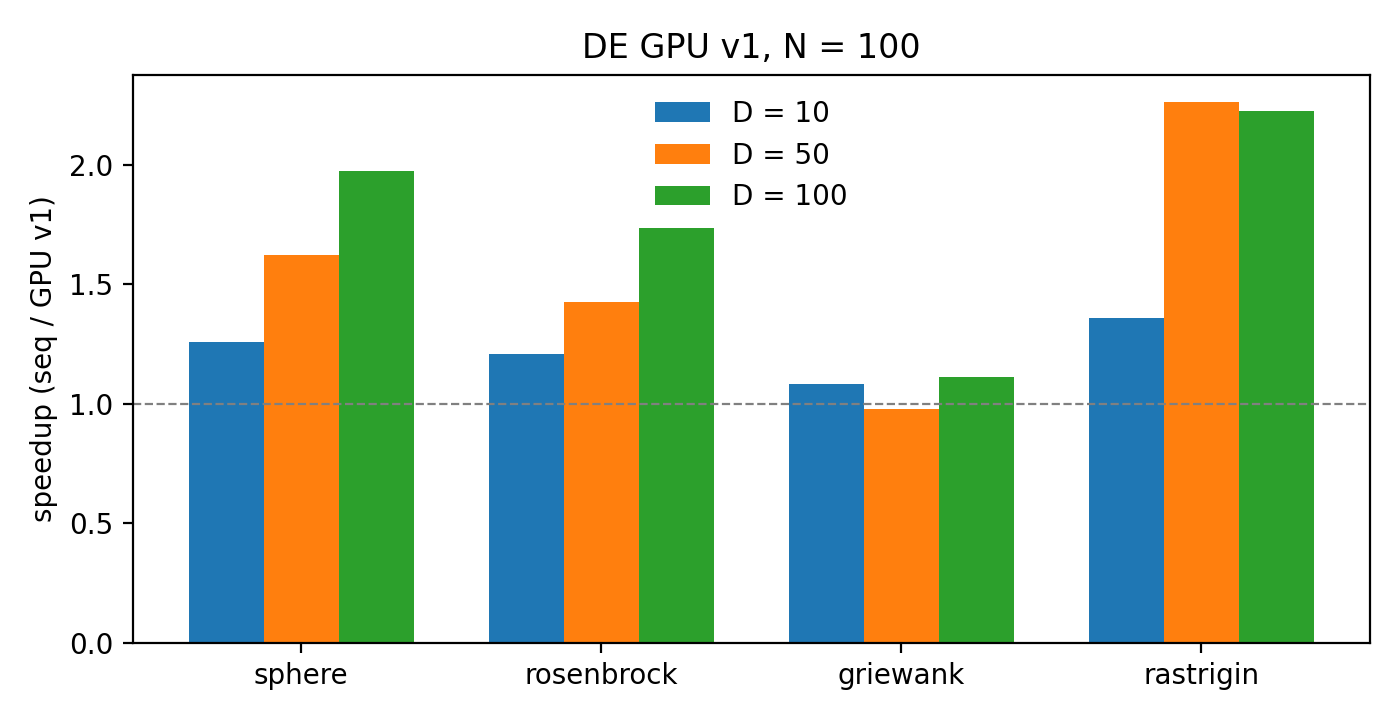
\includegraphics[width=\columnwidth]{speedup_v1.png}
\caption{Speedup of version 1 over the sequential DE ($N=100$).}
\label{fig:sp1}
\end{figure}

\paragraph{Block size and occupancy} For $D=50$ and $D=100$, blocks of 64 to 512
threads all reach 100\,\% theoretical occupancy, yet 128 and 256 threads are always
slower than the best of 32 and 64 (Table~\ref{tab:bloc}): with $D=50$ and $T=256$,
80\,\% of the threads have no gene, and every extra thread lengthens the reduction
and the synchronizations. Small blocks win when the grid already fills the GPU
($N=500$), 64 threads when it does not ($N\le100$). The automatic rule reproduces the
best choice in the 12 measured cases, but it was fitted on these cases; the
threshold $4\times\#\mathrm{SM}=160$ is only known to lie between $N=100$ and $500$,
and the branch $D\le32$ was not swept.

\begin{table}[t]
\centering
\caption{Version 2, Rastrigin: mean time (s, 3 runs) for $T$ threads per block.}
\label{tab:bloc}
\begin{tabular}{rrrrrrr}
\toprule
$D$ & $N$ & 32 & 64 & 128 & 256 & auto\\
\midrule
50  & 50  & 0.1039 & \textbf{0.0913} & 0.1003 & 0.1262 & 0.0912\\
50  & 100 & 0.0535 & \textbf{0.0504} & 0.0587 & 0.0778 & 0.0505\\
50  & 500 & \textbf{0.0205} & 0.0222 & 0.0383 & 0.0818 & 0.0202\\
100 & 50  & 0.2741 & \textbf{0.2194} & 0.2240 & 0.2708 & 0.2198\\
100 & 100 & 0.1421 & \textbf{0.1246} & 0.1376 & 0.1716 & 0.1253\\
100 & 500 & \textbf{0.0599} & 0.0642 & 0.1026 & 0.1704 & 0.0599\\
\bottomrule
\end{tabular}
\end{table}

\paragraph{Version 2 against version 1} Table~\ref{tab:v1v2} and Fig.~\ref{fig:v1v2}.
The gain grows with $D$ ($6.5\times$ to $14.6\times$ for $D=100$). Version~1 was not
tuned (one SM used), so this gain measures the benefit of the gene-level
decomposition rather than an upper bound. No significant difference in quality was
detected between the two versions (Mann--Whitney, 10 runs): Rosenbrock $D=10$
($p=0.623$), Rosenbrock $D=50$ ($p=0.345$), Rastrigin $D=50$ ($p=0.104$). Compared with the
sequential times of Table~\ref{tab:sp1} (Rastrigin, $N=100$), version~2 is about
$4\times$, $22\times$ and $33\times$ faster for $D=10$, $50$ and $100$; these are orders of
magnitude, the sequential times varying by 10 to 17\,\% between runs on Colab.

\begin{table}[t]
\centering
\caption{Mean time (s, 3 runs) of versions 1 and 2, Rastrigin.}
\label{tab:v1v2}
\begin{tabular}{rrrrr}
\toprule
$D$ & $N$ & v1 & v2 & v1/v2\\
\midrule
10  & 50  & 0.0433 & 0.0171 & 2.53\\
10  & 100 & 0.0259 & 0.0088 & 2.95\\
10  & 500 & 0.0054 & 0.0031 & 1.72\\
50  & 50  & 0.7573 & 0.0910 & 8.32\\
50  & 100 & 0.4796 & 0.0504 & 9.51\\
50  & 500 & 0.1014 & 0.0201 & 5.05\\
100 & 50  & 2.7749 & 0.2194 & 12.65\\
100 & 100 & 1.8271 & 0.1249 & 14.63\\
100 & 500 & 0.3864 & 0.0597 & 6.47\\
\bottomrule
\end{tabular}
\end{table}

\begin{figure}[t]
\centering
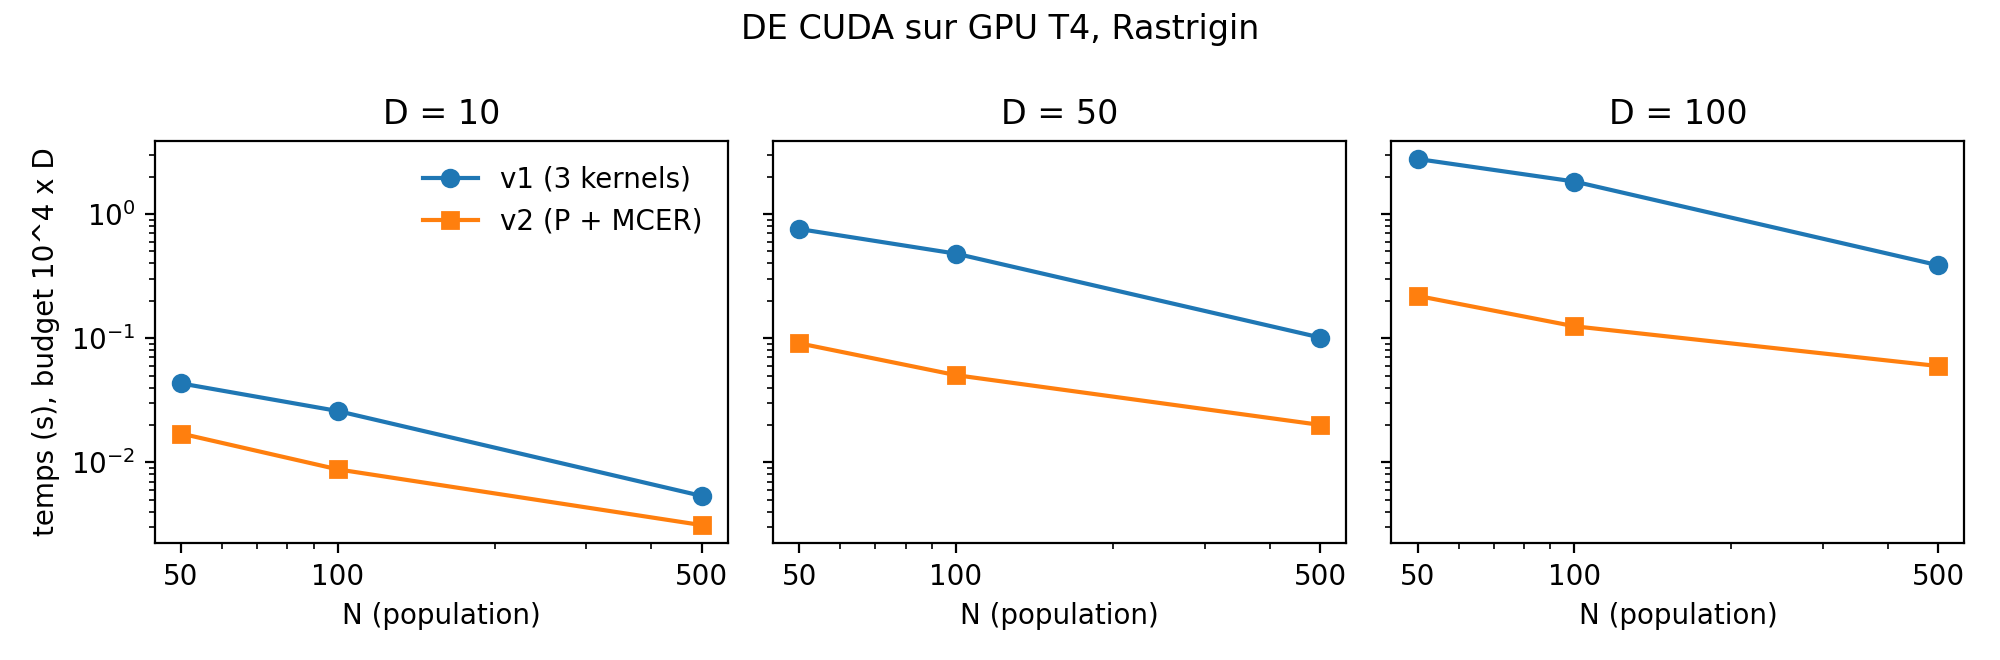
\includegraphics[width=\columnwidth]{temps_v1_v2_N.png}
\caption{Time of versions 1 and 2 as a function of $N$ (Rastrigin, log scales).}
\label{fig:v1v2}
\end{figure}

\paragraph{DE variants} \afaire{Table of the five variants (issue \#17), $D=50$, $N=100$, Kruskal--Wallis and ranking per function.}

\paragraph{Full campaign} \afaire{step 5 (issue \#14): 4 functions $\times$ 3 $D$ $\times$
3 $N$ $\times$ 10 runs for the sequential DE and the GPU versions; quality tables
(mean $\pm$ std per configuration), time and speedup curves (step 6, issue \#16),
Kruskal--Wallis / Wilcoxon tests and comparison with the results of \cite{qin2012}
(issue \#21).}

% =====================================================================
\section{Conclusion}\label{sec:conc}
Mapping one individual to one thread is enough to obtain a correct GPU DE, but not a
fast one: with populations of 50 to 100 individuals, the GPU is almost idle. Mapping
one individual to one block and one gene to one thread, fusing the four DE
operators in a single kernel and keeping the population and the best-individual
search on the device gives a further $1.7\times$ to $14.6\times$ on a Tesla T4, and
about $33\times$ over a sequential implementation (Rastrigin, $D=100$, $N=100$, an order of
magnitude), with no significant difference in quality detected (10 runs, $D\le50$).
Measured timings, not theoretical occupancy, determined the block size.
Limitations: the speedups come from a single GPU and single-core sequential code
compiled with \texttt{-O2}; quality was compared on 10 runs for $D\le 50$ only; the block-size rule was fitted on 12 cases; the
sequential and GPU programs are two variants (asynchronous and generational) of
DE/rand/1/bin. \afaire{conclusions of the full campaign and of the variant study.}

\begin{thebibliography}{10}
\bibitem{storn1997} R.~Storn and K.~Price, ``Differential evolution -- a simple and efficient heuristic for global optimization over continuous spaces,'' \emph{J. Global Optim.}, vol.~11, no.~4, pp.~341--359, 1997.
\bibitem{kennedy1995} J.~Kennedy and R.~Eberhart, ``Particle swarm optimization,'' in \emph{Proc. IEEE Int. Conf. Neural Networks}, vol.~4, Perth, Australia, 1995, pp.~1942--1948.
\bibitem{qin2012} A.~K.~Qin, F.~Raimondo, F.~Forbes, and Y.~S.~Ong, ``An improved CUDA-based implementation of differential evolution on GPU,'' in \emph{Proc. Genetic and Evolutionary Computation Conf. (GECCO)}, 2012.
\bibitem{brest2006} J.~Brest, S.~Greiner, B.~Bo\v{s}kovi\'c, M.~Mernik, and V.~\v{Z}umer, ``Self-adapting control parameters in differential evolution: a comparative study on numerical benchmark problems,'' \emph{IEEE Trans. Evol. Comput.}, vol.~10, no.~6, pp.~646--657, 2006.
\bibitem{salmon2011} J.~K.~Salmon, M.~A.~Moraes, R.~O.~Dror, and D.~E.~Shaw, ``Parallel random numbers: as easy as 1, 2, 3,'' in \emph{Proc. SC11}, 2011, Art.~16.
\bibitem{suganthan2005} P.~N.~Suganthan \emph{et~al.}, ``Problem definitions and evaluation criteria for the CEC 2005 special session on real-parameter optimization,'' Nanyang Technological Univ., Singapore, and KanGAL Rep. 2005005, 2005.
\bibitem{mann1947} H.~B.~Mann and D.~R.~Whitney, ``On a test of whether one of two random variables is stochastically larger than the other,'' \emph{Ann. Math. Statist.}, vol.~18, no.~1, pp.~50--60, 1947.
\bibitem{kruskal1952} W.~H.~Kruskal and W.~A.~Wallis, ``Use of ranks in one-criterion variance analysis,'' \emph{J. Amer. Statist. Assoc.}, vol.~47, no.~260, pp.~583--621, 1952.
\bibitem{wilcoxon1945} F.~Wilcoxon, ``Individual comparisons by ranking methods,'' \emph{Biometrics Bull.}, vol.~1, no.~6, pp.~80--83, 1945.
\bibitem{holm1979} S.~Holm, ``A simple sequentially rejective multiple test procedure,'' \emph{Scand. J. Statist.}, vol.~6, no.~2, pp.~65--70, 1979.
\end{thebibliography}

\end{document}
